\subsubsection{Drivers de potencia}
El control de los tres motores paso a paso se realiza mediante drivers TB6600, que proporcionan control de corriente mediante chopper y aislamiento óptico de señales lógicas. Cada driver opera con tensión de potencia de 24V DC para los motores, y tensión lógica de 5V DC para las señales STEP/DIR/ENABLE.

\underline{Motores NEMA 17 ($\times$2):} Los motores NEMA 17 tienen torque de 0.22 Nm y corriente nominal de 1.8 A por fase. Los drivers TB6600 se configuran mediante DIP switches para limitar la corriente a 1.5 A, protegiendo los motores ante sobrecarga térmica.\\

\underline{Motor NEMA 23 short ($\times$1):} El motor NEMA 23 short tiene corriente nominal de hasta 3.0 A por fase. El driver TB6600 puede entregar hasta 3.5 A, siendo adecuado para este motor. Se configura mediante DIP switches para limitar la corriente a 2.0 A.\\

Los drivers TB6600 operan mediante control PWM (chopper) que regula la corriente efectiva entregada a las bobinas. El consumo de corriente desde la fuente de 24V depende del estado operativo: en reposo con motores energizados el consumo es mínimo (corriente de holding), durante movimiento la corriente aumenta proporcionalmente a la carga mecánica y velocidad, alcanzando valores máximos durante aceleraciones.

\subsection{Reguladores de voltaje}

El sistema emplea dos reguladores DC-DC step-down para adaptar la tensión de alimentación principal (24V DC) a los niveles requeridos por diferentes subsistemas:

\underline{Regulador 24V$\rightarrow$5V (5A):} Regulador conmutado step-down que alimenta:
\begin{itemize}[label=$\bullet$]
\item Arduino Mega 2560 (consumo típico 0.35 A, pico 0.5 A)
\item Raspberry Pi 5 (consumo típico 3.0 A, pico 4.0 A)
\item Cámara USB (consumo típico 0.5 A)
\end{itemize}

\underline{Regulador 24V$\rightarrow$7V (3A):} Regulador conmutado step-down que alimenta:
\begin{itemize}[label=$\bullet$]
\item Servomotores MG996R (2 servomotores) (consumo bajo carga: 0.9 A por servo, pico 1.5 A por servo)
\item Lógica de drivers ($\times$3) (consumo típico 0.3 A)
\end{itemize}

La separación de la alimentación de servomotores respecto a la alimentación de procesadores (5V) previene caídas de tensión causadas por picos de corriente que podrían inducir resets espurios del Arduino.

La Figura \ref{fig:diagrama_voltajes} ilustra el esquema completo de distribución de voltajes desde la fuente primaria de 24V hasta todos los componentes del sistema.

\begin{figure}[H]
\centering
% TODO: Agregar imagen del diagrama de distribución de voltajes
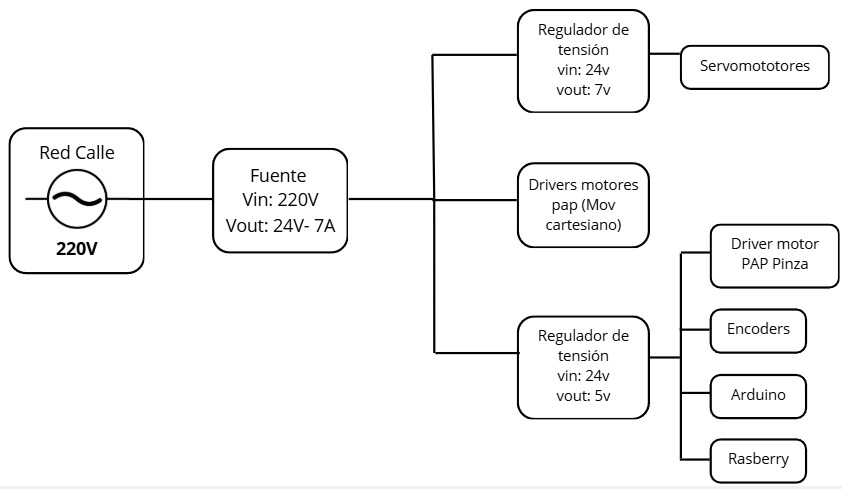
\includegraphics[width=0.75\textwidth]{imagenes/diagrama_voltajes.jpg}
\caption{\textit{Diagrama de distribución de voltajes del sistema mostrando fuente de 24V, reguladores step-down (24V→5V y 24V→7V), y conexiones a todos los componentes}}
\label{fig:diagrama_voltajes}
\end{figure}

\subsection{Análisis energético y dimensionamiento de fuente}

La Tabla \ref{tab:consumo_energetico_prototipo} presenta el consumo eléctrico de cada componente del sistema en diferentes estados operativos, basado en mediciones reales del prototipo.

\begin{table}[H]
\centering
\small
\begin{tabular}{|l|c|c|c|c|}
\hline
\textbf{Componente} & \textbf{Voltaje} & \textbf{Reposo (A)} & \textbf{Operación (A)} & \textbf{Pico (A)} \\
\hline
\multicolumn{5}{|c|}{\textbf{Alimentación 24V}} \\
\hline
Driver TB6600 ($\times$3) & 24V & 0.15 & 1.2 & 1.5 \\
\hline
Regulador 24V$\rightarrow$5V (5A)& 24V & 0.35 & 0.89 & 1.16 \\
\hline
Regulador 24V$\rightarrow$6V (3A)& 24V & 0.05 & 0.52 & 0.83 \\
\hline
\multicolumn{2}{|l|}{\textbf{Subtotal 24V}} & \textbf{0.55} & \textbf{2.61} & \textbf{3.49} \\
\hline
\hline
\multicolumn{5}{|c|}{\textbf{Alimentación 5V (desde regulador 24V$\rightarrow$5V)}} \\
\hline
Arduino Mega 2560 & 5V & 0.2 & 0.35 & 0.5 \\
\hline
Raspberry Pi 5 & 5V & 1.0 & 3.0 & 4.0 \\
\hline
Cámara USB & 5V & 0.3 & 0.5 & 0.5 \\
\hline
\multicolumn{2}{|l|}{\textbf{Subtotal 5V}} & \textbf{1.5} & \textbf{3.85} & \textbf{5.0} \\
\hline
\hline
\multicolumn{5}{|c|}{\textbf{Alimentación 6V (desde regulador 24V$\rightarrow$7V)}} \\
\hline
Servomotores MG996R ($\times$2) & 7V & 0.02 & 1.8 & 3.0 \\
\hline
Lógica drivers ($\times$3) & 6V & 0.3 & 0.3 & 0.3 \\
\hline
\multicolumn{2}{|l|}{\textbf{Subtotal 6V}} & \textbf{0.32} & \textbf{2.1} & \textbf{3.3} \\
\hline
\hline
\multicolumn{5}{|c|}{\textbf{Consumo total en fuente de 24V}} \\
\hline
\multicolumn{2}{|l|}{Reposo} & \multicolumn{3}{c|}{0.55 A @ 24V = \textbf{13 W}} \\
\hline
\multicolumn{2}{|l|}{Operación normal} & \multicolumn{3}{c|}{2.61 A @ 24V = \textbf{63 W}} \\
\hline
\multicolumn{2}{|l|}{Pico máximo} & \multicolumn{3}{c|}{3.49 A @ 24V = \textbf{84 W}} \\
\hline
\end{tabular}
\caption{\textit{Consumo eléctrico del sistema por componente y estado operativo}}
\label{tab:consumo_energetico_prototipo}
\end{table}

Dimensionamiento de la fuente.\\
\noindent
El consumo en operación normal (63 W) ocurre cuando los motores paso a paso están en movimiento continuo bajo carga moderada, los servomotores MG996R operan, y el sistema de visión está procesando imágenes simultáneamente. Los picos de 84 W ocurren durante aceleraciones bruscas con los tres motores paso a paso y los dos servomotores iniciando movimiento simultáneamente bajo carga máxima.

Los valores de consumo de los drivers TB6600 reflejan mediciones reales del sistema: 0.5 A en reposo (motores energizados sin movimiento) y hasta 2.5 A durante operación con todos los motores en movimiento. Esta diferencia respecto al consumo teórico de corriente nominal (5.6 A total) se debe a que los drivers operan mediante control PWM con duty cycle variable, y raramente todos los motores operan simultáneamente a máxima carga.

Se selecciona una fuente conmutada de 24V DC con capacidad nominal de 7 A (120 W), proporcionando un margen de seguridad del 43\% sobre el pico máximo medido. Este margen considera:

\begin{itemize}[label=$\bullet$]
\item Degradación de la fuente con el tiempo (típicamente 10-15\% de pérdida de capacidad tras 2 años de operación continua)
\item Transitorios de corriente durante arranque inicial del sistema
\item Posibles expansiones futuras del hardware (sensores adicionales, iluminación LED, etc.)
\end{itemize}

La eficiencia de los reguladores step-down (90\% para 24V$\rightarrow$5V y 88\% para 24V$\rightarrow$6V) ya está considerada en los cálculos de consumo de la fuente primaria. Las pérdidas totales por conversión de voltaje son de aproximadamente 1.8 W en operación normal (1.0 W en el regulador 24V$\rightarrow$5V y 0.8 W en el regulador 24V$\rightarrow$6V).